% Neural Network Architecture Template
% Multi-layer neural network diagram

\documentclass[tikz,border=10pt]{standalone}
\usepackage{tikz}
\usetikzlibrary{calc,positioning,fit,backgrounds}
\usepackage{amsmath}

\begin{document}
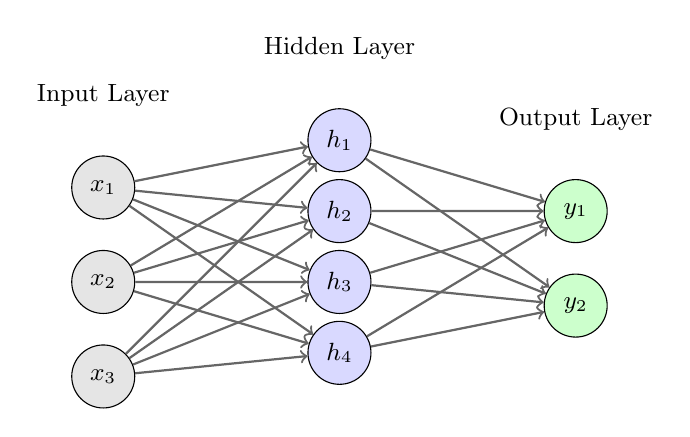
\begin{tikzpicture}[
    node distance=1.2cm,
    font=\small,
    % Layer styles
    input/.style={draw, circle, minimum size=0.8cm, fill=gray!20},
    hidden/.style={draw, circle, minimum size=0.8cm, fill=blue!15},
    output/.style={draw, circle, minimum size=0.8cm, fill=green!20},
    layer/.style={draw, rounded corners=8pt, fill opacity=0.1},
    arrow/.style={->, thick, draw=black!60},
]

    % Input layer
    \foreach \i in {1,2,3} {
        \node[input] (in\i) at (0, -\i*1.2) {$x_\i$};
    }
    
    % Hidden layer
    \foreach \i in {1,2,3,4} {
        \node[hidden] (hid\i) at (3, -\i*0.9 + 0.3) {$h_\i$};
    }
    
    % Output layer
    \foreach \i in {1,2} {
        \node[output] (out\i) at (6, -\i*1.2 - 0.3) {$y_\i$};
    }
    
    % Connections
    \foreach \i in {1,2,3} {
        \foreach \j in {1,2,3,4} {
            \draw[arrow] (in\i) -- (hid\j);
        }
    }
    
    \foreach \i in {1,2,3,4} {
        \foreach \j in {1,2} {
            \draw[arrow] (hid\i) -- (out\j);
        }
    }
    
    % Layer labels
    \node[above=0.5cm of in1] {Input Layer};
    \node[above=0.5cm of hid1] {Hidden Layer};
    \node[above=0.5cm of out1] {Output Layer};

\end{tikzpicture}
\end{document}
